\chapter{Implementacija i korisničko sučelje}
		
		
		\section{Korištene tehnologije i alati}
		
			\text Komunikacija u timu realizirana je korištenjem aplikacija WhatsApp\footnote{\url{https://www.whatsapp.com/}} i Messenger za Facebook\footnote{\url{https://https://www.messenger.com/}}, a sastanci su održavani putem platformi Microsoft Teams\footnote{\url{https://www.microsoft.com/hr-hr/microsoft-365/microsoft-teams/}} te Discord\footnote{url{https://discord.com/}}. Za izradu UML dijagrama korišten je alat Astah UML\footnote{\url{https://astah.net/products/astah-uml/}}, a kao sustav za upravljanje izvornim kodom Git\footnote{\url{https://git-scm.com/}}. Udaljeni repozitorij projekta dostupan je na web platformi GitLab\footnote{\url{https://gitlab.com/}}.
			
			Kao razvojno okruženje korišten je Visual Studio Code\footnote{\url{https://code.visualstudio.com/}} – uređivač koda tvrtke Microsoft. Dostupan je za Window, Linux i macOS. Uključuje podršku za otklanjanje pogrešaka, isticanje sintakse, inteligentno dovršavanje koda, refaktoriranje koda i ugrađeni Git. Inicijalno ima ugrađenu podršku za JavaScript, TypeScript i Node.js, no ima bogat sustav ekstenzija za druge jezike (na primjer C++, Java, Phyton, Dart) i druge radne okvire (.NET, Unity…)
			
			Aplikacija je napisana korištenjem softera Flutter\footnote{\url{https://flutter.dev/}} i programskog jezika Dart\footnote{\url{https://dart.dev/}}. Flutter je softver za razvoj korisničkog sučelja otvorenog koda, razvijen od tvrtke Google. Omogućava višeplatformski razvoj korištenjem jednog koda te jedostavnost izrade aplikacija. Flutter koristi programski jezik Dart, kojim je realiziran i frontend i backend.
			
			Kako bi unutar aplikacije bili omogućeni video pozivi, korišten je Agora RTC\footnote{\url{https://www.agora.io/en/}} servis koji nudi opcije video poziva, glasovnih poziva, live audio i video streaming te slanje poruka.
			
			Baza podataka nalazi se na poslužitelju u oblaku Firestore\footnote{\url{https://firebase.google.com/docs/firestore}}. 
			
			
			
			\eject 
		
	
		\section{Ispitivanje programskog rješenja}
			
			\subsection{Ispitivanje komponenti}
			
			Ispitivanje komponenti verificira rad programskih dijelova koje je moguće neovisno zasebno ispitati. Za ispitivanje smo koristili Flutter Test i MockFirebase priključke.
			
			Kod na slici \ref{fig:addCourse} provodi ispitivanje funkcionalnosti stvaranja tečaja korištenjem funkcije addCourse unutar razreda CoursesDB. U testu su obavljena tri dodavanja tečaja. Nakon toga se provjerava sadrži li kolekcija tri elementa.
			
			\begin{figure}[h]
				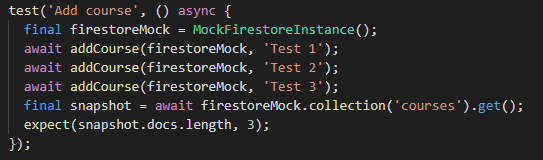
\includegraphics[scale=0.75]{slike/addCourse.PNG}
				\centering
				\caption{addCourse}
				\label{fig:addCourse}
			\end{figure}
			
			Slika \ref{fig:addUniqueUser} prikazuje kod koji provjerava ispravnost dodavanja novog korisnika u bazu podataka pomoću metode addUser. E-mail adrese su jedinstvene unutar baze podataka, odnosno nije dozvoljeno da dva korisnika imaju istu e-mail adresu. Prva dva e-maila su različita i nakon prva dva poziva funkcije addUser dokument bi trebao imati dva elementa. Treći poziv metode sadrži već korištenu e-mail adresu i zbog toga se očekuje da je veličina kolekcije i dalje dva.
			
			\begin{figure}[h]
				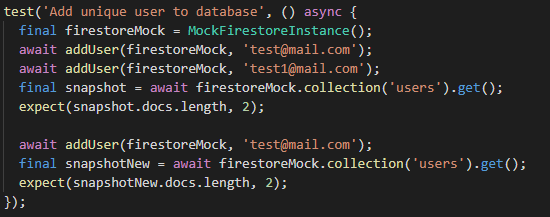
\includegraphics[scale=0.75]{slike/addUniqueUser.PNG}
				\centering
				\caption{Dodavanje novog korisnika}
				\label{fig:addUniqueUser}
			\end{figure}
			
			
			\eject
			
			Kod na slici \ref{fig:noUser} služi za provjeru prijavljenih korisnika. Test očekuje da nema prijavljenih korisnika, tj. da je user jednak null.
			
			\begin{figure}[h]
				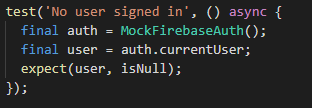
\includegraphics[scale=0.75]{slike/noUser.PNG}
				\centering
				\caption{Provjera prijavljenih korisnika}
				\label{fig:noUser}
			\end{figure}
			
			Prijava korisnika prikazana je na slici \ref{fig:login}. Nakon unosa e-maila i lozinke očekuje se da FirebaseAuth ima prijavljenog korisnika.
			
			\begin{figure}[h]
				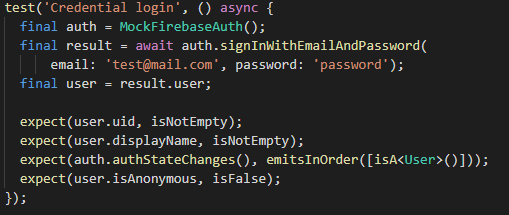
\includegraphics[scale=0.75]{slike/login.PNG}
				\centering
				\caption{Prijava u sustav}
				\label{fig:login}
			\end{figure}
			
			Ispitni slučaj na slici \ref{fig:userFetch} vraća korisnika koji je prijavljen.
			
			\begin{figure}[h]
				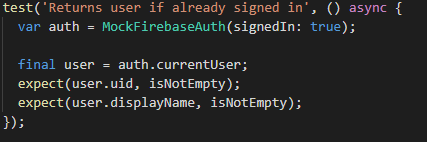
\includegraphics[scale=0.75]{slike/userFetch.PNG}
				\centering
				\caption{Prikaz prijavljenog korisnika}
				\label{fig:userFetch}
			\end{figure}
			
			\eject
			
			
			Kod na slici \ref{fig:signOut} provjerava je li odjava korisnika uspješno provedena.
			
			\begin{figure}[h]
				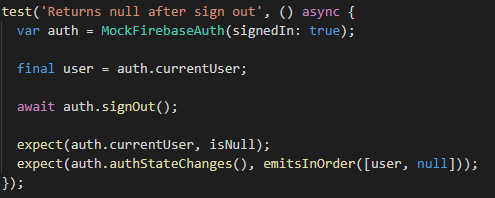
\includegraphics[scale=0.75]{slike/signOut.PNG}
				\centering
				\caption{Provjera odjave}
				\label{fig:signOut}
			\end{figure}
			
			Rezultati testova vidljivi su na slici \ref{fig:unitTests}.
			
			\begin{figure}[h]
				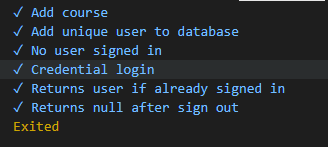
\includegraphics[scale=0.75]{slike/unitTests.PNG}
				\centering
				\caption{Rezultati testova}
				\label{fig:unitTests}
			\end{figure}
			
			Aplikacija je prošla sve testove.
			
			
			\eject
			
			\subsection{Ispitivanje sustava}
			
			Ispitivanje sustava verificira funkcijske i nefunkcijske zahtjeve te prihvatljivost sustava. Automatizirane testove smo proveli pomoću Flutter Drivera.
			
			Ispitni slučaj na slici \ref{fig:wrongCred} simulira pokušaj prijave s neispravnom lozinkom. Nakon unosa e-mail adrese, očekuje se da će se ona nalaziti u svom polju za unos. Jednako tako se očekuje i za lozinku.
			
			\begin{figure}[h]
				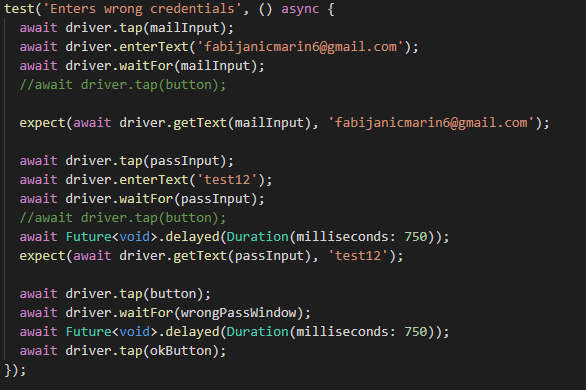
\includegraphics[scale=0.75]{slike/wrongCred.PNG}
				\centering
				\caption{Neispravan unos korisničkih podataka}
				\label{fig:wrongCred}
			\end{figure}
			
			Kod na slici \ref{fig:goodCred} prikazuje prijavu s ispravnom lozinkom. Ovaj put se nakon ponovnog unosa šifre očekuje da će se u polju za unos nalaziti ispravna lozinka, te da će se na pritisak gumba izvršiti prijava.
			
			\begin{figure}[h]
				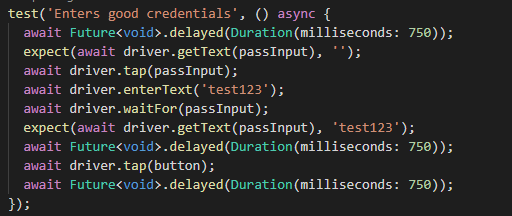
\includegraphics[scale=0.75]{slike/goodCred.PNG}
				\centering
				\caption{Ispravan unos korisničkih podataka}
				\label{fig:goodCred}
			\end{figure}
			
			
			\eject
			
			Kod na slici \ref{fig:wrongName} očekuje da će se, nakon odabira kategorije i težine tečaja, u polju za unos nalaziti naziv tečaja (ovdje je to polje ostavljeno prazno, što se i očekuje). Zatim test očekuje da će se u polju za unos opisa tečaja nalaziti opis, međutim tečaj neće biti dodan jer nije unesen njegov naziv.
			
			\begin{figure}[h]
				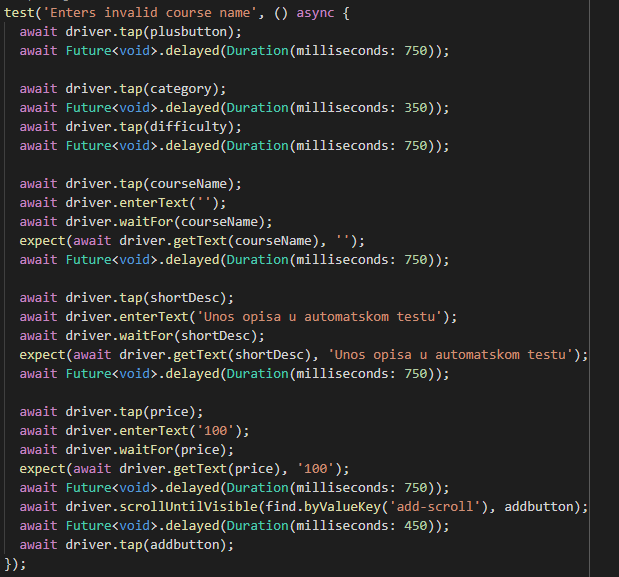
\includegraphics[scale=0.75]{slike/wrongName.PNG}
				\centering
				\caption{Neispravan naziv tečaja}
				\label{fig:wrongName}
			\end{figure}
			
			
			\eject
			
			Kod na slici \ref{fig:validName} očekuje da će se nakon ponovnog unosa naziva tečaja on nalaziti u odgovarajućem polju za unos, te da će se izvršiti dodavanje tečaja.
			
			\begin{figure}[h]
				\includegraphics[scale=0.70]{slike/validName.PNG}
				\centering
				\caption{Unos ispravnog naziva tečaja}
				\label{fig:validName}
			\end{figure}
			
			Slika \ref{fig:editProf} prikazuje kod koji simulira odlazak korisnika na svoj profil i pokušaj izmjene osobnih podataka.
			Korisnik ispravno unosi sve potrebne podatke i uređuje svoj profil. Nakon toga, test se vraća na profilnu stranicu korisnika i provjerava izmijenjene podatke.
			
			\begin{figure}[hbt!]
				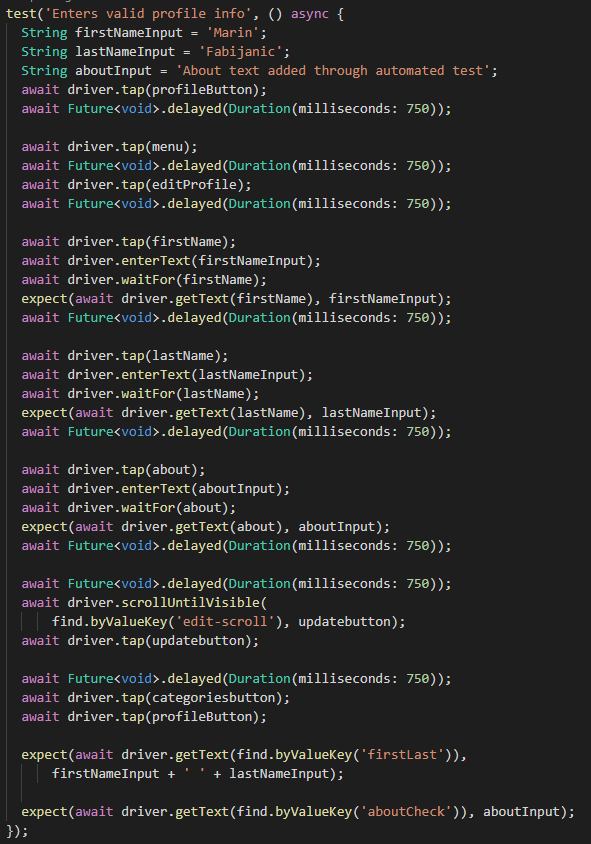
\includegraphics[scale=0.47]{slike/editProf.PNG}
				\centering
				\caption{Uređivanje osobnih podataka}
				\label{fig:editProf}
			\end{figure}
			
			
			\eject
			
			Rezultati testova vidljivi su na slici \ref{fig:integTests}.
			
			\begin{figure}[h]
				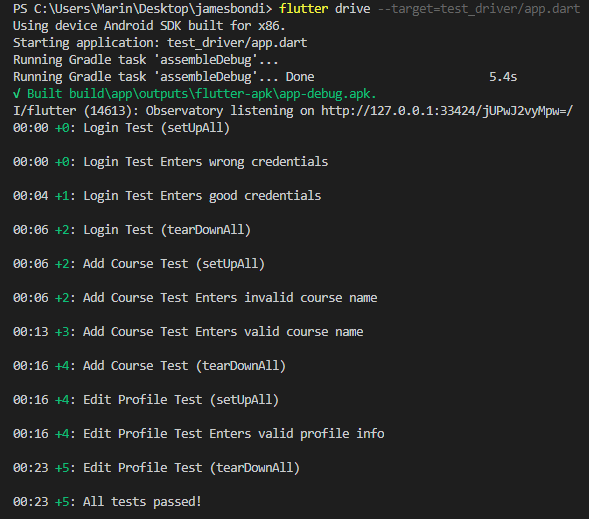
\includegraphics[scale=0.4]{slike/integTests.PNG}
				\centering
				\caption{Rezultati integracijskih testova}
				\label{fig:integTests}
			\end{figure}
			
			Aplikacija je prošla sve testove.
			
			\eject 
		
		
		\section{Dijagram razmještaja}
			
			Dijagram razmještaja opisuje topologiju sustava i usredotočen je na odnos sklopovskih i programskih dijelova. Na slici \ref{fig:Dijagram_razmjestaja} prikazan je specifikacijski dijagram razmještaja koji prikazuje komunikaciju mobilnog uređaja s operacijskim sustavom Android na kojem se nalazi mobilna aplikacija s bazom podataka koja se nalazi u oblaku. Mobilna aplikacija spaja se HTTP protokolom na oblak. U oblaku se unutar Firebase platforme nalazi baza podataka Cloud Firestore, usluga za pohranu podataka Storage i Firebase Authentication za određivanje identiteta korisnika.
			
			
			\begin{figure}[h]
				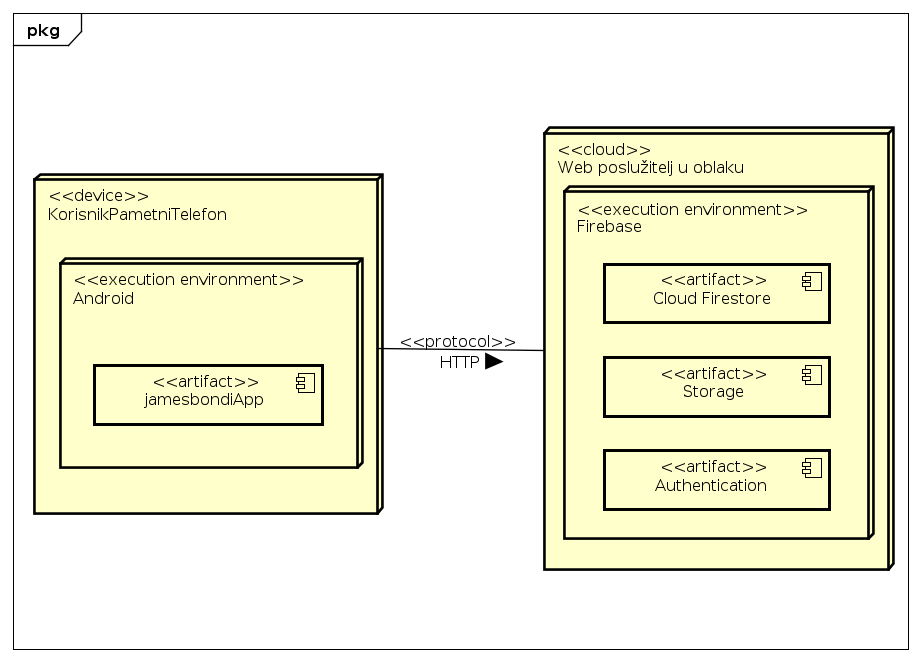
\includegraphics[scale=0.6]{dijagrami/Dijagram_razmjestaja.PNG}
				\centering
				\caption{Dijagram razmještaja}
				\label{fig:Dijagram_razmjestaja}
			\end{figure}
		
			
			\eject 
		
		\section{Upute za puštanje u pogon}
		
			\begin{flushleft}
				\textbf{Postavljanje baze podataka} 
			\end{flushleft}
			
			\text Potrebno je kreirati Firebase račun preko kojega je moguće upravljati svime što je povezano uz bazu podataka. Nakon toga, treba se kreirati Firebase projekt. Kada je stvoren, potrebno je unutar aplikacije spojiti Firebase API preko API ključa i unijeti ID projekta, nakon čega je aplikacija povezana s bazom podataka. 
			
			Nakon toga, potrebno je postaviti Firebase authentication, odnosno omogućiti i postaviti metode za prijavu korisnika. U našem slučaju, jedini mogući način prijave jest putem maila.
			Idući korak u postavljanju naše baze podataka jest inicijalizacija baze podataka na Firestore servisu. Nakon toga, stvara se hijerarhija koja se može vidjeti prethodno u dokumentaciji (slika \ref{fig:ER}).
			
			Zadnji korak je prilagođavanje pravila privatnosti svih Firebase servisa, kako bismo osigurali osjetljive podatke koji će se nalaziti u bazi podataka.
			
			\begin{flushleft}
				\textbf{Postavljanje Agora RTC servisa} 
			\end{flushleft}
		
			\text Kako bi ostvarili mogućnost uspostavljanja video poziva unutar aplikacije, potrebno je bilo kreirati račun na servisu Agora. Nakon stvaranja računa, stvoren je novi projekt te je tako dobiven poseban AppID koji smo povezali s našom aplikacijom.  
			
			\begin{flushleft}
				\textbf{Izgradnja Android aplikacije} 
			\end{flushleft}
			
			\text Za izgradnju Android aplikacije u Flutteru, prvo je potrebno promijeniti ikonu. Nakon toga, potrebno je digitalno potpisati aplikaciju, odnosno generirati ključ kojeg zatim treba referencirati u posebnoj datoteka. Idući korak jest uređivanje build.gradle datoteke kako bi konfigurirali digitalni potpis aplikacije. Nakon toga, potrebno je App Manifest datoteku i build.gradle datoteku prilagoditi sukladno uputama na \textit{\href{https://flutter.dev/docs/deployment/android}{poveznici}} te  zatim kreirati APK datoteku. 
			
			\begin{flushleft}
				\textbf{Puštanje Android aplikacije u pogon} 
			\end{flushleft}
			
			\text Za puštanje naše aplikacije u pogon, odabrali smo servis \href{https://developer.getjar.mobi/}{Getjar}. Kao i za prethodne servise, i za ovaj je bilo potrebno stvoriti račun. Nakon toga, bilo je potrebno uz APK datoteku priložiti i ime aplikacije, detaljan opis, snimke zaslona i tome slično kako bi aplikacija prošla pregled od strane servisa. Aplikacija je također submitana na Amazon App trgovinu. 
			\eject
			\begin{figure}[h]
				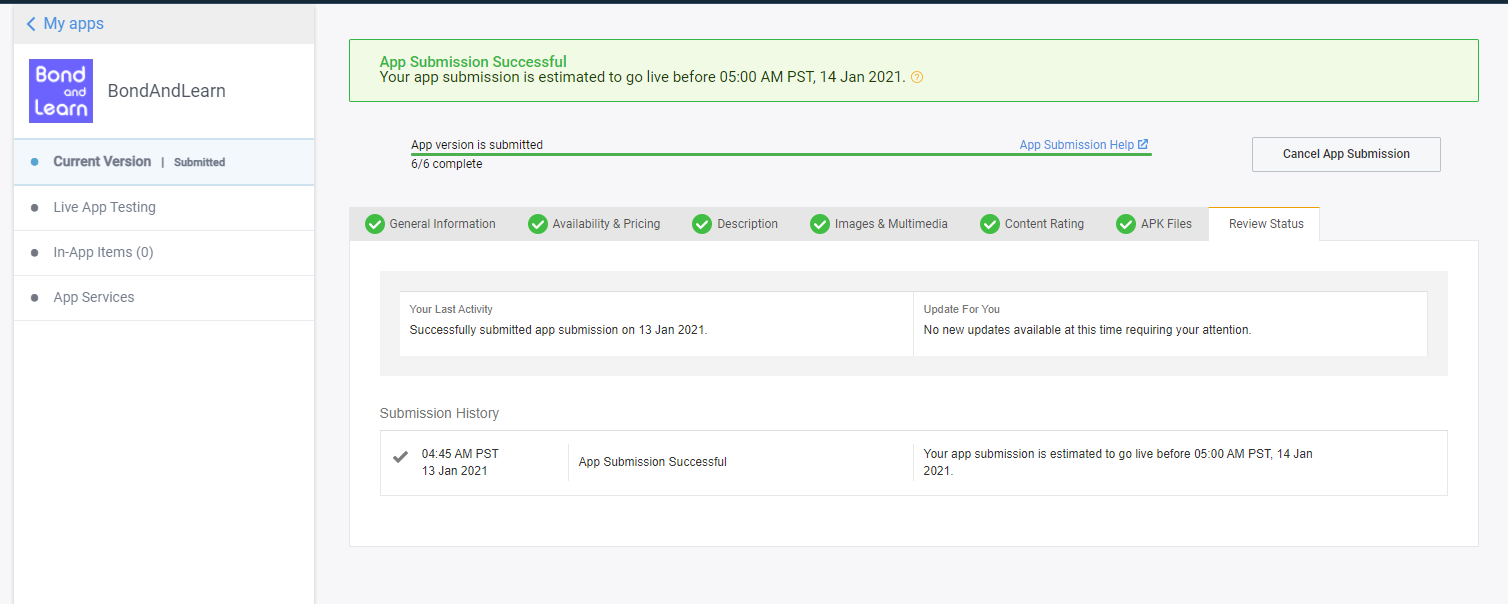
\includegraphics[scale=0.3]{slike/Getjar.PNG}
				\centering
				\caption{Status aplikacije na Getjar servisu}
				\label{fig:Getjar}
			\end{figure}
			
			\begin{figure}[h]
				
\includegraphics[scale=0.2]{slike/Amazon.JPEG}
				\centering
				\caption{Status aplikacije na Amazon App trgovini}
				\label{fig:Amazon}
			\end{figure}
			
			\eject 